\documentclass[11pt]{report}
% packages
% Fran Burstall's Bath thesis package
\usepackage{baththesis}
\usepackage{amssymb} %for Blackboard bold etc \usepackage{graphicx} %for including eps graphics % front matter
\usepackage[pdftex]{graphicx} % To include pictures
\usepackage{caption}
\usepackage{subcaption} % To use subfigures with subcaptions
\usepackage{url}
\usepackage{amsmath} % Equations
\usepackage{txfonts}
\setlength{\parskip}{0.9em} %Paragraph spacing
\usepackage{pgfgantt}
\usepackage{cite}
\usepackage{csquotes}
\renewcommand*{\mkcitation}[1]{ #1}

\newcommand{\phim}{\mathbf{\phi}}
\newcommand{\X}{\mathbf{X}}
\newcommand{\x}{\mathbf{x}}
\newcommand{\Y}{\mathbf{Y}}
\newcommand{\y}{\mathbf{y}}
\newcommand{\w}{\mathbf{w}}
\newcommand{\Z}{\mathbf{Z}}
\newcommand{\z}{\mathbf{z}}
\newcommand{\h}{\mathbf{h}}
\newcommand{\dd}{\: \mathrm{d}}

%\usepackage[hidelinks]{hyperref} % Adds references links without color
\usepackage{hyperref} % Adds references links with color
\usepackage{xcolor}
\hypersetup{
    colorlinks,
    linkcolor={red!50!black},
    citecolor={blue!50!black},
    urlcolor={blue!80!black}
}

\title{Visual Effects} \author{Ieva Kazlauskaite, Garoe Dorta-Perez, Richard Shaw}
%\degree{Doctor of Philosophy}
\unit{ unit }
\department{Department of Computer Sciences} \degreemonthyear{May 2015}
\norestrictions

\begin{document}
\maketitle

\chapter{Introduction}
\label{ch:intro}
\begin{center}
\textquote[~\cite{Attenborough:1998}]{\textit{Birds are the most accomplished aeronauts the world has ever seen. They fly high and low, at great speed, and very slowly. And always with extraordinary precision and control}.}
\end{center}


\chapter{Previous Work}
\label{sec:previous}

\section{Data Capture}

%-----------------------------------------------------------------------
\section{Sparse Reconstruction}


%-----------------------------------------------------------------------
\section{Blendshape Optimisation}
In this section we introduce the techniques used to warping the meshes and the optimisation methods.

\subsection{Thin Plate Splines}
Thin plate theory deals with problems that commonly arise in areas of natural sciences and engineering when trying to model the behaviour of a thin sheet of some material. The possible processes include but are not limited to stretching, bending, crumpling, buckling, shrinking, straining and tearing. The corresponding mathematical model is based on ideas from differential geometry, and the set of equations describing the aforementioned phenomena are often notoriously difficult to solve. Therefore, in Computer Graphics, as well as other fields, a number of simplifying assumptions are made when constructing a thin plate model. \\

A thin plate is considered to be a two dimensional object, i.e. it is assumed that the thickness is infinitesimal. The geometry of the object is often simplified to reduce the computational cost. Thin plate splines (TPS) are a two-dimensional counterpart of the cubic spline. TPS are a deformation method based on the assumption that a thin surface deforms in a way that minimises the surface bending energy. The bending energy is proportional to the change in the second fundamental form. Specifically, given two corresponding sets of point $\{\y_i\}_i^N$ and $\{\x_i\}_i^N$ there exists a height field mapping between the two, $f: \mathbb{R}^2 \to \mathbb{R}$. The bending energy corresponding to this mapping is proportional to the second order derivatives of the mapping:
\begin{equation}
\begin{aligned}
	E_{bend}(f) = \lambda \iint \left( \left( \dfrac{\delta^2f}{\delta x^2} \right)^2 +  2 \left( \dfrac{\delta^2f}{\delta x y} \right)^2 +  \left( \dfrac{\delta^2f}{\delta y^2} \right)^2 \right) \dd x \dd y,
\end{aligned}
\end{equation} where $\lambda$ is smoothing parameter, which balances the quality of fit and the amount of bending, i.e. the wiggliness of the function. TPS finds the transformation that fits the data while minimising the bending energy. Note that TPS may also be defined in terms of the radial basis functions that are used for smooth scattered data fitting. The RBF solution for thin plate splines is:
\begin{equation}
\begin{aligned}
	f(x) = \sum_{i=1}^N \alpha_i \: \phi(\|\x - \x_i\|), \: \text{ where} \: \phi(r) = r^2 \log(r).
\end{aligned}
\end{equation} 

\subsection{Non-Rigid ICP}


\subsection{Numerical Solvers}



%-----------------------------------------------------------------------
\section{Skin Rendering}

Rendering realistic skin is a challenging task.
As social beings, we interact with each other on a daily basis, humans perception is quite sensitive to skin appearance, specially with faces.
Skin is composed of several layers with different properties, to accurately simulate skin, the light transport between this layers has to be modelled.
The full effect of light scattering between two points on the surface can be modelled using a Bidirectional Surface-Scattering Distribution Function (BSSRDF).

Weyrich et al~\cite{Weyrich2006} proposed a two-layer model for skin rendering, the outer layer simulates the air-oil interface and the inner layer models the subsurface scattering in the skin.
The authors scattering to be homogeneous, with this assumption they measured the skin BRDF of several subjects with a light dome, while the scattering was sampled at three points in the face with a sensor head with a linear fiber array.
The BRDF data was fitted to a Blinn-Phong and a Torrance-Sparrow isotropic models, while the scattering was fitted with a single transport coefficient.
Donner et al~\cite{Donner2008} also proposed a two-layer model, however the authors allow for the layers to be heterogeneous.
With this addition they are able to introduce the effects of haemoglobin, veins and tattoos.
Emotional induced haemoglobin variations have also been explored ~\cite{Jimenez2010}.
The authors measured the haemoglobin distributions of several subjects in different poses, then a linear combination of the captured data would determine the final haemoglobin distribution for a new sequence.
Recently, Iglesias et al~\cite{Iglesias2015} introduced a five-layer model to handle skin ageing.
Haemoglobin, collagen and fat changes with age are modelled using the different layers.

Normal maps are use to alter the normals of the scene objects during rendering.
This technique is used to add geometric detail to an object at rendering time without actually changing the geometry.
The error introduced with this approach is shown in Figure \ref{fig:normal_map}, a ray $r_1$ hist the geometry at point $p$ and the normal $n_p$ is used for shading, while if we had the based geometry the hitting point would be $p'$ and the normal $n'$.
Normal maps are for skin rendering are usually captured using expensive light domes with a number of synchronized cameras ~\cite{Graham2013, Weyrich2006}. 

Another techniques to increase the quality of a face render is to the resolution of the textures being used.
Hertzmann et al~\cite{Hertzmann2001} proposed a filter to synthesize images based on a neighbour search given a pair of samples images.
Al alternative technique using a dictionary of samples was presented by Jianchao et al~\cite{Jianchao2010}, the authors was limited to generation of increased resolution images.
Graham et al~\cite{Graham2013} applied Hertzmann et al~\cite{Hertzmann2001} example based filter to generate higher quality bump maps for skin rendering.
For an in depth analysis of super-resolution techniques, we refer the reader to Tian et al \cite{Tian2011} survey.

\begin{figure}[htbp!]
\centering
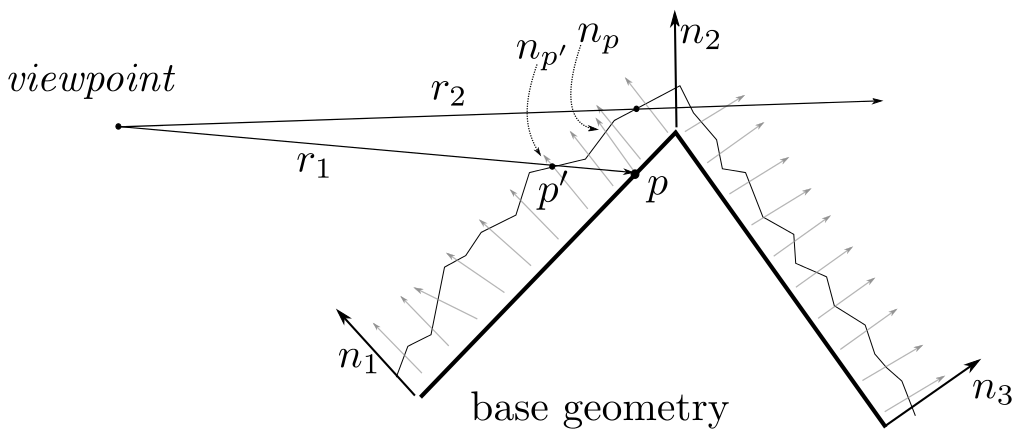
\includegraphics[width=0.7\textwidth]{img/normal_map}
	\caption{ Using normal maps to simplify a given geometry, image taken from \cite{ganovelli2014}.}
	\label{fig:normal_map}
\end{figure}



%-----------------------------------------------------------------------
\chapter{Methodology}
\label{sec:methods}


\section{Data Capture}


\section{Sparse Reconstruction}


\section{Blendshape Optimisation}


\section{Skin Rendering}

\cite{Hertzmann2001} Image analogies paper.


%-----------------------------------------------------------------------
\chapter{Results}


%-----------------------------------------------------------------------
\chapter{Conclusions}

\bibliographystyle{eg-alpha}
\bibliography{baththesis}

\end{document}